\ifx\wholebook\relax\else
\input{../Common.tex}
\input{../macroes.tex}
\begin{document}
\fi
\chapter{Conditions}\label{cha:condition}\label{cha:conditional}

Up until now the programs we defined \replace{were executing}{executed} \textit{all} the \replace{messages that composed them}{expressions they contained,} one after the other. We had no way to \replace{define}{say} that certain messages \replace{could}{should} only be executed \replace{when certain}{in some} situations\replace{ were met}{, but not in others}. \replace{In this}{This} chapter and the \replace{following one we}{next} introduce an important programming concept: the notion of \emph{conditional} \index{condition} execution, \replace{\ie\}{i.e.} the fact \add{that} a certain piece of code \replace{is executed}{executes only} when a \replace{given}{specified} condition \replace{holds}{is true}. 

\replace{We start by defining}{This chapter starts with} a simple problem that shows the need \replace{of}{for} conditional execution\replace{, then we present in detail}{. Then it presents} the conditional expressions available in \st\add{ in detail}.

\section{A Simple Problem}

\replace{We would like}{Suppose you want} to change the color of a robot depending on its distance from the center of the screen. \replace{Let us say that if}{If} a robot is \replace{located at a distance smaller}{less} than 200 pixels from the center\add{,} it should be red\replace{ else}{; otherwise} it should be green. This problem requires \replace{a \textit{conditional}}{conditional} execution. \replace{Indeed depending}{Depending} on \replace{the robot}{a condition --- the robot's} location \add{---} its color should \replace{be different.}{change. \paragraph
}
The method \ct{distanceDetector} shows a possible solution\add{,} and \Tscrref{scr:detector} \replace{presents a possible scenario showing}{shows} how the method \ct{distanceDetector} \replace{is}{can be} used. @@dank: Would 'setColor' be a better name? or  'setColorForDistance'? or 'setTwoColors' for parallelism with the nesting example later in this chapter?@@

\begin{scriptwithtitle}{A Simple Detector}\label{scr:detector}
\caro := \Turtle new. 
\caro jump: 20.
\caro distanceDetector.
\caro jump: 200.
\caro distanceDetector.
\end{scriptwithtitle}


\begin{method}\label{mth:detector}
distanceDetector
   | dist | 
   dist := self distanceFrom: World center.
   dist < 200
      ifTrue: [self color: Color red]
      ifFalse: [self color: Color green]
\end{method}
@@dank: I suggest rearranging the material to introduce ifTrue: first.  It is simpler and easier to explain than ifFalse: and ifTrue:ifFalse:.  Then you could cover ifFalse: and finally ifTrue:ifFalse:.  I think that most students would learn with less effort that way. Then the above script would be:
	setColor
		| distanceFromCenter |
		self color: Color green.
		distanceFromCenter := self distanceFrom: World center.
		(distanceFromCenter < 200)
			ifTrue: [self color: Color red].
@@
	

\replace{Let us}{Let's} analyze \remove{now} what happens when the expression \ct{\caro distanceDetector} is executed. 

\begin{enumerate}
\item The expression \ct{self distanceFrom: World center} computes the distance from the receiver to the center of the screen. This distance is stored into the variable \ct{dist}. 

\item Then the expression \ct{dist < 200 ifTrue: [self color: Color red] ifFalse: [self color: Color green]} is executed as follows: \textit{if} the distance is smaller than 200\add{,} the color of the receiver is changed to red\replace{ else}{; otherwise} it is changed to green. This expression is a \textit{conditional} expression. \add{(It is spread over three lines in the method definition but it is all one expression, because there is no period to terminate it earlier.)}
 
\end{enumerate}

\begin{figure}[h]
\begin{center}
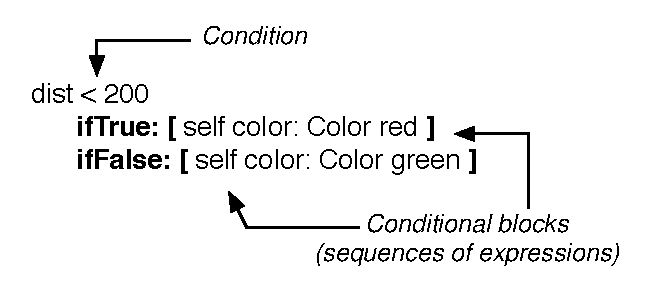
\includegraphics{distanceDetector}
\caption{A conditional expression \add{is} composed of a condition and conditional messages.
@@dank: Would it be more consistent with previous usage to call them 'conditional blocks' instead of messages?  This would also avoid ambiguous meanings of the plural: sometimes 'conditional messages' might refer to both the true & false branches, other times to multiple messages in one branch. 'Block' would make it easier to distinguish. This change should then propagate throughout the chapter, though I have marked it only in a few places; if you accept the change, I will revise accordingly.@@\label{fig:distanceDetector}}
\end{center}
\end{figure}

A conditional expression is composed of two parts: a \index{condition}\textit{condition} and \index{conditional messages} \textit{conditional messages}. 
The expression \ct{dist < 200} is a condition and the expressions \ct{[self color: Color red]} and \ct{[self color: Color green]} are conditional messages\add{,}  as shown by Figure~\ref{fig:distanceDetector}.   

The method \ct{ifTrue:ifFalse:} executes one condition, here \ct{dist < 200}, and depending of its value, executes \add{one of} the \add{conditional} messages \replace{corresponding to the true or the false case}{and skips the other}. The keyword \ct{ifTrue:} indicates that the conditional message \ct{[self color: Color red]} is only executed when the condition \add{\ct{dist < 200}} is true. Similarly the keyword \ct{ifFalse:} indicates that  the conditional message  \ct{[self color: Color green]} is only executed when the condition is false.

\replace{What you see is that}{So} there are different kinds of expressions. Some such as \ct{self distanceFrom: World center} are always executed\add{,} while others are executed only when their \replace{associate}{associated} condition \replace{hold.}{holds. \paragraph
}
\replace{Note that a}{Each} conditional \replace{expression}{message is a block enclosed in square brackets \ct{[ ]}. A block} is not limited to \replace{one}{a} single \replace{message}{expression,} but can \replace{be}{contain} a \replace{composition of messages as presented in Chapter~\ref{cha:boolean}}{series of statements as you saw in Chapter~\ref{cha:variables}}. The method \ct{ifTrue:ifFalse:} defines two possible executions\add{,} which can \add{each} contain \replace{complex}{a} sequence of messages.  \add{\paragraph
}
Note that the method \ct{ifTrue:ifFalse:} is a \textit{single} method with two arguments, one for the true case and one for the false case. \replace{Therefore you should not}{If you} put a period \replace{after the \ct{]} following the \ct{ifTrue:}}{before the \ct{ifFalse:} part, it will break the conditional statement by ending it too soon, causing an error}.


When we presented how to define methods in Chapter~\ref{ch:turtleTeaching} we explained that executing a method not only evaluates the messages it contains\add{,} but also returns a value. 
Up until now we \replace{did}{have} not really used the result returned by \replace{methods}{a method}. \replace{Now for the condition expression 
we are essentially interested by}{But for some conditional expressions,} the result returned by \replace{the}{a} method\add{ is essential}. For example in method \ref{mth:detector}, the expression  \ct{self distanceFrom: World center} not only computes the distance of the receiver from the center of the screen but \add{also} \textit{returns} \replace{it}{that distance}.  The condition expression, \ct{dist < 200}, uses this value to decide \replace{wich}{which} branch \replace{should be executed}{to execute}. 

@@dank: Is ifFalse:ifTrue: important? Since this is an introductory textbook, not a reference, I recommend omitting it entirely (along with the related figure and following paragraphs) as a rarely-used feature. It offers little to a beginner but an opportunity for confusion. @@
\paragraph{\ct{ifTrue:ifFalse} and \ct{ifFalse:ifTrue:}.}
The method \ct{ifFalse:ifTrue:} also exists. It works the same way the method \ct{ifTrue:ifFalse:}, \ie it executes the false case when the condition is false and the true one when the condition is true, exactly as the method \ct{ifTrue:ifFalse:}. This method is just \remove{there} to help you \replace{writing}{write} more readable code if you want to start \replace{reading}{with} the messages executed when the condition is false as shown by Figure~\ref{fig:conditionalifTifFifFifT}.


\begin{figure}[h]
\begin{center}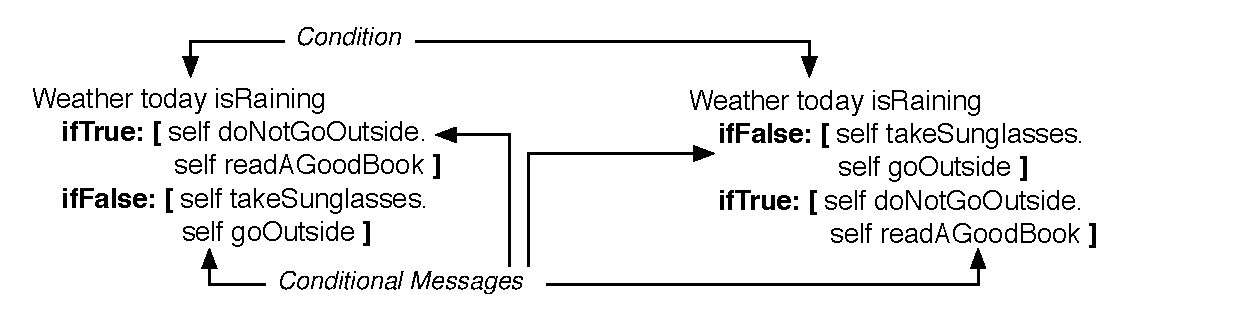
\includegraphics[width=\linewidth]{conditionalifTifFifFifT}
\caption{Two equivalent \replace{conditionals}{conditional} expressions.\label{fig:conditionalifTifFifFifT}}\end{center}
\end{figure}




\fprod{production the following should be in a frame}
A conditional expression is composed of two parts: a \index{condition}\textit{condition} and \index{conditional messages} \textit{conditional messages}. 

\begin{nalltt}
\textit{aCondition}
\quad \textbf{ifTrue: [} \textit{messagesIfConditionIsTrue}\textbf{]}
\quad  \textbf{ifFalse: [} \textit{messagesIfConditionIsFalse} \textbf{]}

\textit{aCondition}
\quad   \textbf{ifFalse: [} \textit{messagesIfConditionIsFalse} \textbf{]}
\quad   \textbf{ifTrue: [} \textit{messagesIfConditionIsTrue} \textbf{]} 
\end{nalltt}
\fprod{until here}


\section{Two Other Conditional Messages: \ct{ifTrue:} and \ct{ifFalse:}}

Sometimes we only need to perform \replace{one}{an} action when a \replace{given}{specific} condition is true\add{,} but \add{do} nothing when the condition is false \add{(} or vice versa\add{)}. For example the method \ct{redWhenCloseToCenter} (\ref{mth:redWhenCloseToCenter}) only changes the color of the receiver to red when it is at a distance smaller than 200 pixels from the screen center.

\begin{method}\label{mth:redWhenCloseToCenter}
redWhenCloseToCenter
   | dist | 
   dist := self distanceFrom: World center.
   dist < 200
      \bold{ifTrue: [}self color: Color red \bold{]}
      \bold{ifFalse: []}
\end{method}

Using the method \ct{ifTrue:ifFalse:} we just have to leave the second branch empty \ie\ \ct{[]}. However, \st provides two other methods \remove{\ct{ifTrue:} and \ct{ifFalse:}} to express \replace{this kind}{these kinds} of conditional expressions\add{: \ct{ifTrue:} and \ct{ifFalse:}}. The method \ct{ifTrue:} executes its conditional messages when its condition is true. Using the method \ct{ifTrue:} we rewrite the method \ct{redWhenCloseToCenter} shown in \ref{mth:redWhenCloseToCenter} as shown in \mthref{mth:redWhenCloseToCenter2}.

\begin{method}\label{mth:redWhenCloseToCenter2}
redWhenCloseToCenter
   | dist | 
   dist := self distanceFrom: World  center.
   dist < 200
      \bold{ifTrue:} [self color: Color red]
\end{method}

Contrary to \ct{ifTrue:}, the method \ct{ifFalse:} executes its conditional messages when its condition is \emph{false}. The methods \replace{\ct{ifFalse:}}{\ct{ifTrue:}} and \ct{ifFalse:} both execute a condition and\add{,} depending on the value returned by the condition, \add{either} execute or \replace{not}{skip} the conditional messages. \add{\paragraph
}
@@dank: Are the next paragraph and related figure important? I recommend omitting them, and treating this topic along with boolean expressions.@@
Note that we can always negate \add{(logically reverse)} a condition to \replace{pass}{switch} from one form to the other. \replace{As shown}{For example} in method~\ref{mth:redWhenCloseToCenter3}, \ct{dist >= 200} is the negation of the expression \ct{dist < 200}. 

\begin{method}\label{mth:redWhenCloseToCenter3}
redWhenCloseToCenter
   | dist | 
   dist := self distanceFrom: World  center.
   \bold{dist >= 200}
      \bold{ifFalse:} [self color: Color red]
\end{method}


\fprod{production the following should be in a frame}
The method \ct{ifTrue:} executes its conditional messages when its condition is true.
The method \ct{ifFalse:} executes its conditional messages when its condition is false.

\begin{nalltt}
\textit{aCondition}
      \textbf{ifTrue: [} \textit{messagesIfConditionIsTrue} \textbf{]}

\textit{aCondition}
      \textbf{ifFalse: [} \textit{messagesIfConditionIsFalse} \textbf{]}
\end{nalltt}
\fprod{until here}

@@dank: I recommend cutting the next paragraph from the book, as it is not essential to beginners.  It is a special type of logic error that doesn't seem more important than other logic errors that haven't been singled out for similar treatment.  If it is included, the explanation should be expanded with two pairs of illustrative examples: one pair where ifTrue:ifFalse is logically equivalent to ifTrue: and ifFalse:, and another pair where it is logically different.  If you decide to keep this topic, I could draft an extended explanation and examples for your review and revision. @@
\paragraph{A Subtle Point.}  The difference between using \ct{ifTrue:ifFalse:}\add{,} and \ct{ifTrue:} followed by \ct{ifFalse:} \add{using the same condition,} is that the \textit{condition} using \ct{ifTrue:ifFalse:} is only executed once, while with \ct{ifTrue:} followed by \ct{ifFalse:} the conditions of the two conditional expressions are executed twice. This can be a problem when \add{the} conditional messages of the first conditional expression (\ct{ifTrue:}) \replace{modifies}{modify} what is tested by the condition of the second conditional expression (\ct{ifFalse:}). In such a case using \ct{ifTrue:} followed by \ct{ifFalse:} is not equivalent to using \ct{ifTrue:ifFalse:}.



\section{Nesting Conditional Expressions}
A conditional expression can contain any other messages and in particular other conditional expressions. This is what we \replace{present now}{demonstrate next}. There is nothing spectacular \add{about it,} but it is common \add{--- and} that is 
why we want to show it to you. Conditions can be nested inside conditions.

\paragraph{Another Simple Problem.}
\replace{Let us}{Let's} modify \replace{our}{the} previous problem. Now \remove{we would like that} if a robot is \replace{located at a distance smaller}{less} than 200 pixels from \replace{a point}{the center,} it should be red\replace{,}{;} when it is between 200 and 300 pixels \add{away,} it should be yellow\add{;} and at a distance greater than 300\add{,} it should be green.  Figure~\ref{fig:detector} shows various robots that \replace{changed}{set} their color using the method \ct{threeColorDetector}. @@dank: Would 'setThreeColors' be a better name?@@

@@dank: This figure is missing from my copy of BookBasicLevel.pdf.@@
\begin{figure}
\begin{center}
\includegraphics[width=10cm]{detector}
\caption{Various robots at different distances from a point. \label{fig:detector}}
\end{center}
\end{figure}

\replace{What we see from our}{In this} problem\replace{ is that}{,} different parts of the method should be executed under different circumstances\replace{ changing the}{. The} color \add{should change} to yellow \remove{should be performed} under \add{different} conditions \remove{that are different} than \add{for} changing the color to green. A possible solution to our problem is shown by method \ref{mth:threeColorDetector}. 

@@dank: I recommend skipping this copy and just using the mth:detector4 version.  I don't think this one adds any value, and it complicates the references in the text.@@
\begin{method}\label{mth:threeColorDetector}
threeColorDetector
   | dist | 
   dist := self distanceFrom: World  center.
   dist > 300
      ifTrue: [self color: Color green]
      ifFalse: [dist < 200
         ifTrue: [self color: Color red]
         ifFalse: [self color: Color yellow]]
\end{method}

@@dank: If you keep both versions (mth:threeColorDetector and mth:detector4), I recommend inserting some explanation about the relationship at the beginning of the next paragraph, for instance "\tmthref{mth:detector4} contains the exact same code with highlighting added to show the conditional expressions."@@ 
\replace{We have}{There are} two different \replace{conditions that we hilighted}{conditional expressions in this method. The first is shown} in italics\add{,} and \add{the second} in bold \remove{as shown explicitly below} in \tmthref{mth:detector4}\add{ (below)}. The second \replace{condition}{conditional expression} (in bold) is only executed \replace{whether}{when} the condition of the first \replace{one}{conditional expression} is false. \replace{Here when}{When} the distance is smaller than 300\replace{ the condition}{, conditional expression} 2 is executed\replace{ which}{. That} means \remove{that} its condition is executed and\replace{ that}{,} depending on its values\add{,} the \replace{right}{correct} branch is executed. If you have \replace{problem to identify this}{trouble identifying the} two \replace{conditionals}{conditional expressions}, \replace{take a colored pen and for one}{pick some} particular value \replace{of}{for} the distance\replace{,}{ (like 150, 250, or 350). Then take a colored pen and} underline the part of \replace{the}{each} method that will be executed\replace{, you will see}{. Following each step carefully will show} that only certain branches are executed. 


\noindent
\begin{minipage}[l]{8cm}
\begin{method}\label{mth:detector4}
threeColorDetector
   | dist | 
   dist := self distanceFrom: World  center.
   \textit{dist > 300
      ifTrue: [self color: Color green]
      ifFalse: [}\textbf{dist < 200
         ifTrue: [self color: Color red]
         ifFalse: [self color: Color yellow]}\textit{]}
\end{method}
\end{minipage}
\hspace{1cm}
\begin{minipage}[r]{8cm}
\begin{nalltt}
\textrm{\replace{Condition}{Conditional Expression} 1:}
\textit{dist > 300
      ifTrue: [self color: Color green]
      ifFalse: [ ... ]}

\textrm{\replace{Condition}{Conditional Expression} 2:}
\textbf{dist < 200
         ifTrue: [self color: Color red]
         ifFalse: [self color: Color yellow]}
\end{nalltt}
\end{minipage}



%%%%%%%%%%%%%%%%%%%%%%%%%%%%%%%%%%%%%%%%%%%%%%%%%%%%%%%%%%%%%
\section{Learning from Errors}
As \replace{we}{people} are always \replace{doing errors}{making mistakes} , looking at errors is an excellent way to learn and understand \add{a concept} from another perspective\remove{ a concept}.  \replace{We defined the method}{Method} \ct{coloredTurn: anAngle} \remove{that} changes the color of a robot \replace{is relation with}{according to} the direction \remove{to which} it is heading\remove{ at}. \replace{We decided that when}{When} the robot \replace{was pointing}{points} to the north it should \replace{become}{turn} blue to represent cold\replace{,}{.  It should turn} red when \replace{pointing to the the}{it points} south\replace{ else}{, and otherwise} it should be green. Our first \replace{definition of}{try at defining} this method is \replace{presented}{shown} in~\tmthref{mth:colored}. \remove{This definition is not correct. Try to understand why before reading the following. }

\begin{method}\label{mth:colored}
coloredTurn: anAngle
     "change the color of the robot so that it is blue aiming 
     at the north and red to the south"
     self turn: anAngle.
     self direction = 90
         ifTrue: [self color: Color blue].
     self direction = -90
         ifTrue: [self color: Color red]
         ifFalse: [self color: Color green]
\end{method}

\add{The above definition is not correct. Try to understand why before reading any farther. }

\replace{This}{The above} method is wrong because when the robot is pointing to the north\add{,}  its color is green\replace{ while}{. But} it should be blue\add{,} as shown in \tscrref{scr:illustbug} and \tscrref{scr:bug}.  

\begin{scriptwithtitle}{Illustrating the bug}\label{scr:illustbug} 
| \caro |
\caro := \Turtle new.
\caro coloredTurn: -90.
\caro color \pr  Color red           "ok"
\caro coloredTurn: 90.
\caro color \pr Color green.      "ok"
\caro coloredTurn: 90.
\caro color \pr Color green      "wrong"
\end{scriptwithtitle}


\paragraph{Why...} Execute \remove{mentally} ~\tmthref{mth:colored} \replace{and}{mentally to} identify why this method is wrong. \replace{In fact the}{The} problem is that even if the condition  \ct{self direction = 90} is true and \remove{that} its associated block is executed, the method continues and evaluates the false conditional \add{message} of the last conditional \replace{statement}{expression}, changing \remove{then} the color of the robot to green\replace{ as shown by the following illustration}{. The following commented version of the code illustrates this}.


\begin{nalltt}
\caro coloredTurn: 90.

   self direction = 90 \textrm{\add{"}is true}
       \textrm{so the true \replace{conditional message}{branch} is executed\add{:"}} ifTrue: [self color: Color blue]
       \textrm{\add{"}the robot becomes blue and we evaluate the \replace{following}{next conditional expression:"}}
   self direction = -90 \textrm{\add{"}is false} 
       \textbf{\textrm{so the false \replace{conditional message}{branch} is executed\add{:"}} ifFalse: [self color: Color green]}
\end{nalltt}


\paragraph{The solution...} To solve our problem we have to be sure that all the code follows the right conditions\add{,} and in particular that certain code is not executed\add{ in other specific conditions}. \replace{Hence, we have to}{To accomplish this,} nest code under the correct condition as shown in the method~\ref{mth:correctcoloredTurn}.

\begin{method}\label{mth:correctcoloredTurn}
coloredTurn: anAngle
   "change the color of the robot so that it is blue \replace{aiming at the}{when pointing}  
   north\replace{ and}{,} red \replace{to the}{for} south, \add{and} green \replace{else}{otherwise}"
   self turn: anAngle.
   self direction = 90
      ifTrue: [self color: Color blue]
      ifFalse: [ self direction = -90
         ifTrue: [self color: Color red]
         ifFalse: [self color: Color green]]
\end{method}

\section{Interpreting a \replace{Mini Language}{Mini-Language}}

@@dank: I agree that this section should be omitted, or moved after introducing boolean expressions.  I've skipped reviewing the commented-out text for now; it will need review if it is ever included.@@
%\paragraph{Wider coloring.}
% We would like to change the color of a robot to blue when its direction is between 45 and 125 degrees, red when it is pointing between -45 and -125. \Tmthref{mth:fuzzycolored} shows you one possible solution. The use of the method \index{between:and:}\ct{between:and:} provides a readable way to express certain conjunction. 
%\ct{5 between: 0 and: 10} is equivalent to \ct{(5<10) \& (5>0)}.

%\begin{method}\label{mth:fuzzycolored}
%coloredTurn: anAngle
%   "change the color of the robot so that it is blue aiming at 
%   the north and red to the south"
%   self turn: anAngle.
%   (self direction between: 45 and: 125)
%      ifTrue: [^self color: Color blue].
%   (self direction between: -45 and: -125)
%      ifTrue: [^self color: Color red].
%   self color: Color green
%\end{method}


In \add{theoretical} biology\remove{ theory}, researchers \add{have} developed systems called Lindermeyer systems \replace{that allows them to study}{for studying} the growth of plants. Lindermeyer systems are based on \replace{turtle}{robot} graphics similar to the robot we use. In addition \remove{the idea is that} the robot understands a \replace{mini language}{mini-language} \replace{constituted by characters}{composed of character codes} such as \ct{\$g} and \ct{\$t}. A robot action is associated \replace{to}{with} each of these \replace{characters}{character codes}. For example the character \ct{\$g} is associated with \replace{move}{moving} forward\add{,} and \ct{\$t} \replace{to turn of}{with turning} 45 degrees. A Lindermeyer system generates a list of \replace{characters  that}{these codes.  The characters} are then interpreted by the \replace{turtle}{robot,} and \replace{this produces}{the actions it takes produce} pictures. \add{\paragraph
}
Define the method \ct{interpret: aCharacter} that \replace{make}{makes} the robot \add{either} move forward when the character is \ct{\$g}\replace{ and}{, or} turn 45 \replace{degree}{degrees} when the character is \ct{\$t}\remove{ as illustrated in the \scrref{src:interpret}}. \Tscrref{src:interpret} illustrates how this method is used.

\begin{scriptwithtitle}{Using \ct{interpret: aCharacter}}\label{src:interpret}
| \replace[2]{pica}{\caro} |
\replace[2]{pica}{\caro} := \Turtle new. 
4 timesRepeat: 
   [ \replace[2]{pica}{\caro}  
       interpret: $g;
       interpret: $t;
       interpret: $g; 
       interpret: $g;
       interpret: $t;
       interpret: $g ]
\end{scriptwithtitle}

The method \ct{interpret:} can be defined \replace{as follows}{this way}:

\begin{method}\label{mth:interpret}
interpret: aCharacter
   aCharacter = $g
      ifTrue: [self go: 20]
      ifFalse: 
         [aCharacter = $t
            ifTrue: [self turn: 45]]
\end{method}

Try to define reproduce \remove{the} Figure~\ref{fig:interloops}. \add{\paragraph
}
@@dank: The next sentence is a forward reference --- I suggest omitting it, or (assuming cha:collection will exist) moving the reference to a separate section at the end of the chapter.@@
We will build a complete \replace{lindermeyer}{Lindermeyer} system in \add{\charef{cha:collection}} when we \remove{will} explain collections. 

%Note that this method will be reused in \tcharef{cha:collection} in which we will show how to use collections as shown in the script~\ref{scr:fun} and illustrated simply in figure ~\ref{fig:interloops}.

%\begin{scriptwithtitle}{Using interpret: in a \replace{loops}{loop}}\label{scr:fun}
%| \caro |
%\caro := \Turtle new.
%'gttgttgttttttgttttttgttgttgttttttgttttttg' 
%	 do: [:aChar | \caro interpret: aChar]
%\end{scriptwithtitle}

\begin{figure}
\begin{center}\includegraphics{interpretLoops}
\caption{A picture generated using the method \ct{interpret:} with the sequence of characters 'gttgttgttttttgttttttgttgttgttttttgttttttg'. \label{fig:interloops}}
\end{center}
\end{figure}

\paragraph{Further Experiments.} Enhance the method \ct{interpret: aCharacter} so that \add{either} \$g or \$G 
\replace{makes}{will make} the robot \replace{goes}{go} forward\add{,} and \replace{that}{either} \$t or \$T \replace{makes}{will make} it \replace{turns}{turn 45 degrees}. \replace{Add also that}{Also add the codes}  \$+ \replace{makes}{to make} the robot
 \replace{turning}{turn} left\add{,} and \$- \add{to turn} right. 









\section{Summary}

\begin{itemize}
\item A conditional expression is composed of two parts: a \index{condition}\textit{condition} and \index{conditional messages} \textit{conditional messages}. 
\end{itemize}

\begin{table}[h]
\small
\centering
\begin{tabular}{||p{8cm}|p{7cm}||} \hline
Method&Description\\ \hline
\begin{nalltt}
\textit{aCondition} 
   ifTrue: [ \textit{messagesIfConditionIsTrue} ]
\end{nalltt}&Execute messagesIfConditionIsTrue only if aCondition is true. \add{\paragraph
Example:} If \replace{a}{the} robot is pointing to the north, it turns green.

\begin{nalltt}
self direction = 90
   ifTrue: [ self color: Color green ]
\end{nalltt}\\  \hline

\begin{nalltt}
\textit{aCondition} 
   ifFalse: [ \textit{messagesIfConditionIsFalse} ] 
\end{nalltt}&Execute messagesIfConditionIsFalse only if aCondition is false.  \add{\paragraph
Example:} The system beeps only when the robot is not pointing to the north. 

\begin{nalltt}
self direction = 90 
   ifFalse: [ \stbeep ]
\end{nalltt} \\ \hline

\begin{nalltt}
\textit{aCondition}
   ifTrue: [ \textit{messagesIfConditionIsTrue} ]
   ifFalse: [ \textit{messagesIfConditionIsFalse} ]
\end{nalltt}&Execute messagesIfConditionIsTrue \replace{whether}{when} aCondition is true\add{;} otherwise execute messagesIfConditionIsFalse. \add{\paragraph
Example: If the robot is pointing to the north, it turns green; otherwise the system beeps.}

\begin{nalltt}
self direction = 90 
   ifTrue: [self color: Color green ]
   ifFalse: [ \stbeep ]
\end{nalltt}\\  \hline
\begin{nalltt}
\textit{aCondition} 
   ifFalse: [ \textit{messagesIfConditionIsFalse} ]
   ifTrue: [ \textit{messagesIfConditionIsTrue} ]
\end{nalltt}&Execute messagesIfConditionIsTrue \replace{whether}{when}  aCondition is true\add{;} otherwise execute \replace{messagesIfConditionIsTrue}{messagesIfConditionIsFalse}. \replace{The robot pick a diamond when it can otherwise the system beeps.\add{\paragraph
Example: If the robot is pointing to the north, it turns green; otherwise the system beeps.}

\begin{nalltt}
self direction = 90 
   ifFalse: [ \stbeep ]
   ifTrue: [ self color: Color green ]
\end{nalltt} \\ \hline
\end{tabular}
\end{table}



\ifx\wholebook\relax\else\end{document}\fi





